\documentclass{article}

\usepackage{Packages_Makros}

\MyTitle{Portfolio}
\MySubtitle{Die Energiewirtschaft}
\MyAuthor{Felix Hehemann}
\MyEmail{felix.hehemann@fh-muenster.de}
\MyMatrNo{1250378}
\MyDepartment{Energie Gebäude Umwelt}
\MyFirstExaminer{Prof. Dr. Peter Vennemann}

\begin{document}

\myMakeTitlepage

\section{Energienutzung in der Zivilisationsgeschichte}
    \begin{figure}[h]
    \centering
    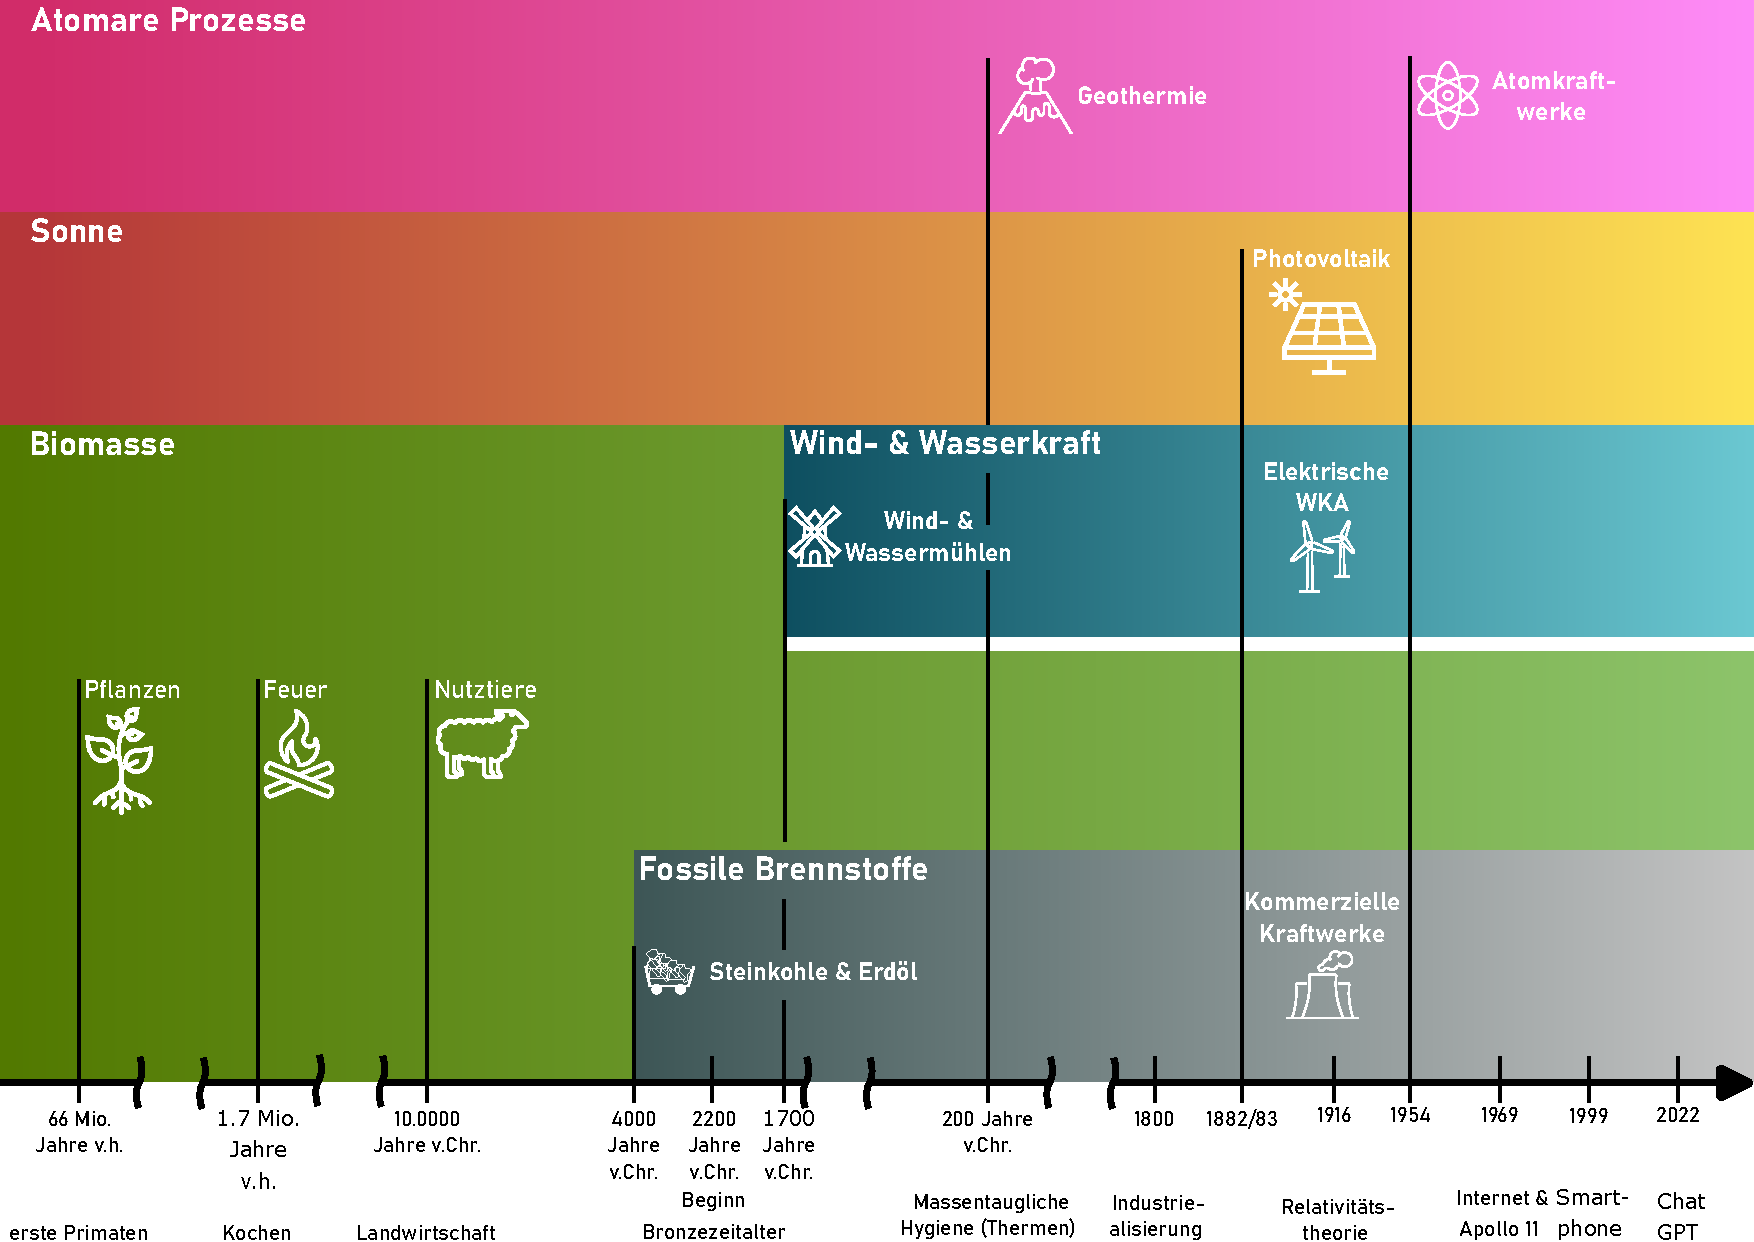
\includegraphics[width=1\linewidth]{Abbildungen/Zivilisation_Energie.pdf}
    \caption[Genutzte Energiequellen in der Zivilisationsgeschichte]{Die Abbildung zeigt unterschiedliche genutzte Energiequellen in der Zivilisationsgeschichte der Menschheit sowie Zusammenhänge mit technischem und gesellschaftlichem Fortschritt. Aus dem hierarchischen Aufbau wird deutlich, dass mit wachsendem Fortschritt immer mehr und höherwertige Quellen erschlossen wurden.}
    \label{fig:Energienutzung}
\end{figure}

\begin{table}[]
    \centering
    \begin{tabular}{c|p{10 cm}}
         Ereignis &  Quelle  \\
         \hline
        erste Primaten & \url{ https://geoundnatur.de/Documents/geologische-zeitskala.pdf} \\
        \hline
        Pflanzen & \url{https://geoundnatur.de/Documents/geologische-zeitskala.pdf}  \\
        \hline
        Feuer & \url{https://doi.org/10.1086/203705}, \url{https://doi.org/10.1073/pnas.1117620109} \\
        \hline
        Kochen & \url{https://doi.org/10.1073/pnas.1107806108} \\
        \hline
        Nutztiere & \url{https://www.youtube.com/watch?v=xiYMWSA3s\_A} \\
        \hline
        Wind- \& Wassermühlen & Golding, E. W. (1976). The Generation of Electricity by the Wind, reprinted with additional material by E. \& FN Spon.; Quaschning, V. (2015). Regenerative Energiesysteme: Technologie-Berechnung-Simulation. Carl Hanser Verlag GmbH Co KG. \\
        \hline
        Steinkohle- \& Erdölnutzung & \url{https://10.1126/sciadv.adh0549} \\
        Bronzezeitalter -\& & \url{https://geoundnatur.de/Documents/geologische-zeitskala.pdf} \\ 
        Geothermie & Bundesverband Geothermie \\
        \hline
        Industrialisierung & \url{https://de.wikipedia.org/wiki/Industrialisierung}  \\ 
        \hline
        Kommerzielle Kraftwerke & Wolter, D., \& Reuter, E. (2005). Preis-und Handelskonzepte in der Stromwirtschaft: von den Anfängen der Elektrizitätswirtschaft zur Einrichtung einer Strombörse. Springer-Verlag. \\
        \hline
        Elektrische WKA & \url{https://www.e-rara.ch/zut/22499137 }\\
        \hline
        Photovoltaik & \url{https://doi.org/10.2475/ajs.s3-26.156.465} \\
        \hline
        Relativitätstheorie & \url{https://doi.org/10.1007/978-3-540-87777-6\_1}\\
        \hline
        Atomkraftwerke &  \url{https://www.iaea.org/newscenter/news/obninsk-beyond-nuclear-power-conference-looks-future}\\
        \hline
        Internet \& Apollo 11 & \url{https://www.nasa.gov/mission/apollo-11/}; \url{https://www.deutschlandfunk.de/erste-nachricht-im-arpanet-vor-50-jahren-als-der-100.html}\\
        \hline
        Chat GPT & \url{https://openai.com/de-DE/index/chatgpt/}
    \end{tabular}
    \caption{Quellen zu \ref{fig:Energienutzung}}
    \label{tab:placeholder}
\end{table}

\end{document}
